\chapter{Abordări din literatură}
\label{Capitolul 3}
Tehnologia de tip deepfake, ajutată de progresul rapid al modelelor adânci, precum Rețelele Generative Adversariale(GAN), au avut in impact semnificativ în sfera digitală prin crearea de conținut sintetic realistic. Acest avans în tehnologie reprezintă un adevărat pericol pentru confidențialitatea, securitatea și integritatea informației. Din acest motiv, este nevoie de mecanisme robuste pentru detecție a conținutului nelegitim. 

În ultimii ani, diverse lucrări din literatură au abordat această temă folosind inteligență artifcială, dar și tehnici tradiționale bazate pe verificarea inconsistențelor din imagini/videoclipuri. Atenția va fi acordată performanțelor pe bazele de date Celeb-DF \cite{li2020celeb} și FaceForensics++ \cite{rössler2019faceforensics}, întrucât lucrarea prezentată folosește date din aceste două seturi.

\section{Celeb-DF (Celebrities Deepfake)}

Introdusă de Li et al. (2020) \cite{li2020celeb}, Celeb-DF este o bază de date vastă care a devenit un nou etalon pentru detecția de conținut fabricat. A fost proiectată cu scopul de a aduce progres în acest câmp de cercetare, abordând mai multe limitări ale seturilor de date anterioare, precum DeepFakeTIMIT \cite{khan2021adversarially} și FaceForensics++ \cite{rössler2019faceforensics}, oferind videoclipuri deepfake de înaltă calitate și diversitate. Celeb-DF conține 5639 de videoclipuri fabricate de rezoluție înaltă generate folosind o metodă, ce minimizează artefactele de compresie și sporește realismul expressiilor și mișcărilor faciale. 

Un aspect important al acestei baze de date, este faptul că videoclipurile conțin secvențe cu celebrități, un grup de persoane care are șanse mult mai mari să apară în conținut de tip deepfake.

Pe lângă videoclipurile fabricate, setul de date include și un set divers de videoclipuri originale, oferind astfel un mediu de antrenare propice. Intorducerea Celeb-DF a contribuit semnificativ la dezvoltarea tehnicilor de detectare a deepfake-urilor.

\begin{figure}[htbp]
    \centering
    \begin{minipage}[b]{0.45\textwidth}
        \centering
        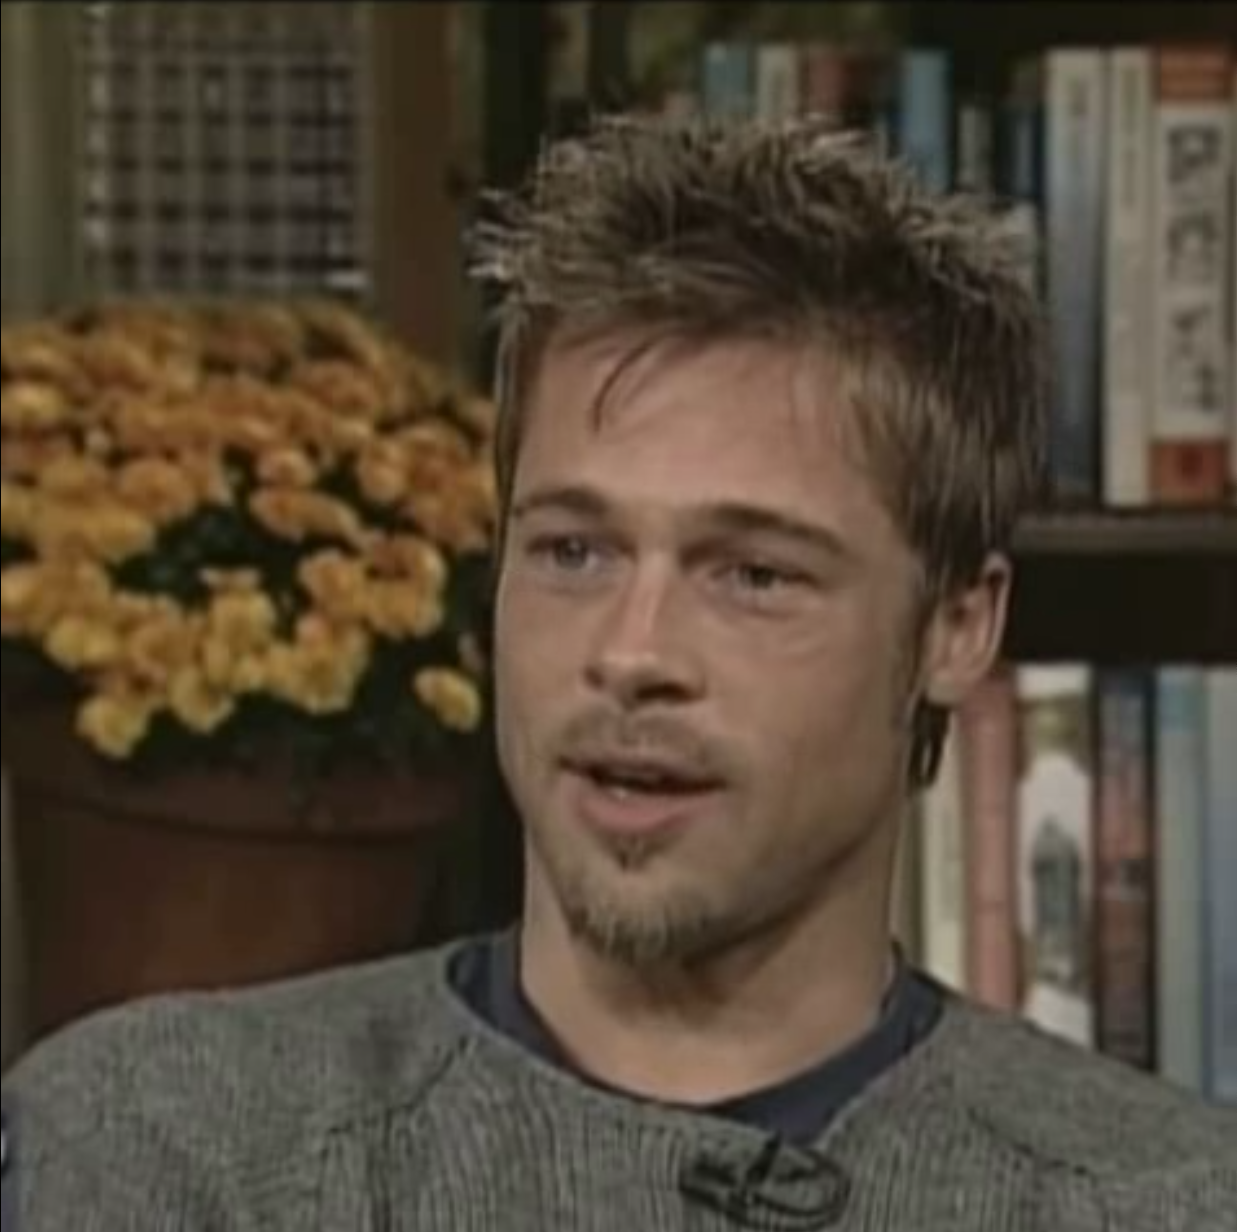
\includegraphics[width=\textwidth]{images/brad-pitt_real.png}
        \caption{Captură dintr-un videoclip original cu actorul Brad Pitt}
    \end{minipage}
    \hfill
    \begin{minipage}[b]{0.45\textwidth}
        \centering
        
\includegraphics[width=\textwidth]{images/brad-pitt_df.png}
        \caption{Captura dintr-un videoclip DeepFake}
    \end{minipage}
\end{figure}

Autorii lucrării au testat riguros pe setul de date diferite modele performante în detecția de deepfake-uri, scoțând în evidență robustețea dar și slăbiciunile lor. Dintre acestea, 2 modele s-au remarcat prin performanța lor.

\begin{itemize}
    \item \textbf{XceptionNet}\cite{rössler2019faceforensics}\cite{Chollet_2017_CVPR}: bazată pe modelul Inception(\cite{szegedy2015going}), această arhitectură s-a dovedit a fi foarte puternică pentru task-uri de clasificare. A fost adaptata pentru detecția de deepfake-uri, datorită capabilităților sale de feature extraction. XceptionNet s-a dovedit a se descurca în particular bine la detecția artefactelor introduse în timpul creării deefake-ului, obținând o acuratețe de 65.5\%.

    \newpage
    \begin{figure}[h]
         \centering 
         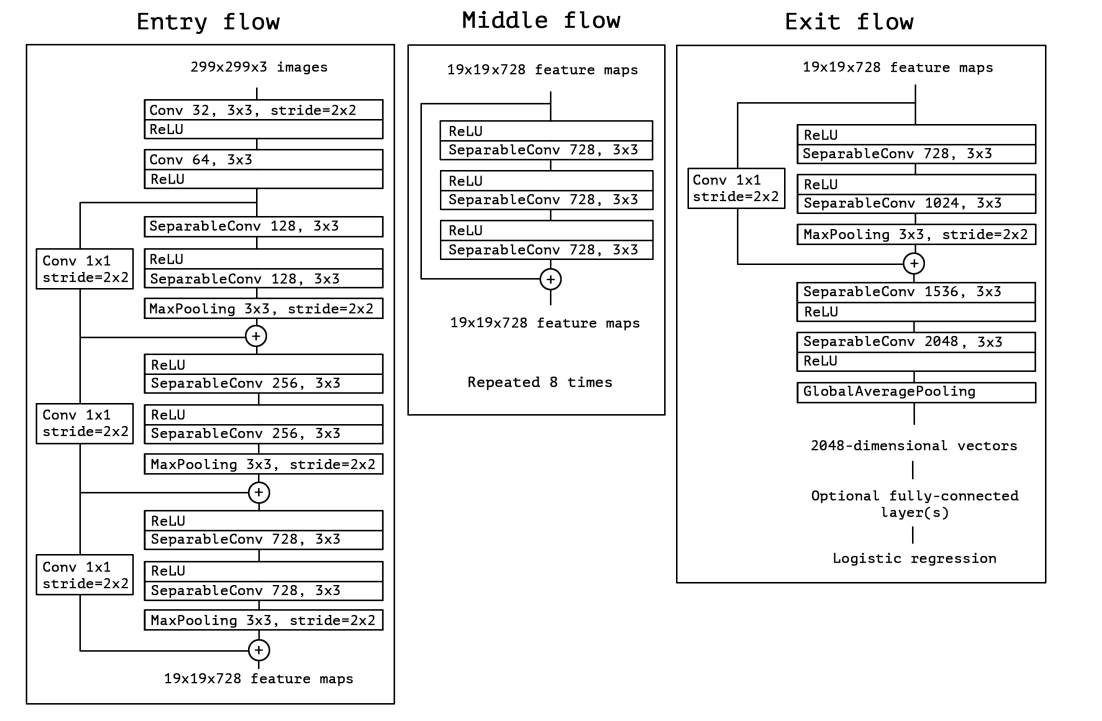
\includegraphics[width=0.85\linewidth]{images/xception-architecture.png}
         \captionsetup{font=footnotesize}
         \caption{Arhitectura Xception \cite{Chollet_2017_CVPR}}
    \end{figure}
    
    \item \textbf{Face Warping Artifacts}\cite{zhou2018twostream}: Modelul Face Warping Artifacts(FWA)este conceput pentru a detecta artefactele de distorsionare a feței, frecvent întâlnite în videoclipurile deepfake. Aceste artefacte sunt distorsiuni subtile introduse în timpul procesului de manipulare a feței, care pot include structura facială nenaturală sau inconsistențe în textură. Combinat cu alte tehnici de detecție a deepfake-urilor, modelul combinat DSP-FWA(DeepFake Stack Pointer Face Warp Artifacts) a obținut o performanță de 64.6\%.
\end{itemize}

\begin{figure}[h]
     \centering 
     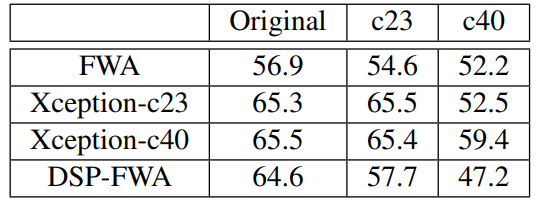
\includegraphics[width=0.5\linewidth]{images/celeb-df_results.png}
     \captionsetup{font=footnotesize}
     \caption{Rezultatele pentru diferite modele \cite{li2020celeb}}
\end{figure}


\section{FaceForensics++}

FaceForensics++ este un set de date și o platformă de benchmark esențială în cercetarea detectării deepfake-urilor și a altor tipuri de conținut deepfake. Dezvoltat de Andreas Rössler și colegii săi, FaceForensics++ a fost conceput pentru a oferi o resursă cuprinzătoare și diversă pentru antrenarea și evaluarea algoritmilor de detectare a conținutului fabricat. 

FaceForensics++ include peste 1,000 de videoclipuri de înaltă calitate, preluate din diferite surse și manipulate folosind mai multe tehnici avansate. Aceste videoclipuri sunt împărțite în patru categorii principale ce reprezintă algoritmii folosiți pentru crearea deepfake-urilor:

\begin{itemize}
    \item \textbf{Deepfakes}: Videoclipuri manipulate folosind tehnici de deepfake, care implică substituirea feței unei persoane cu cea a altei persoane folosind rețele generative adversariale (GANs).
    \item \textbf{Face2Face}\cite{thies2016face2face}:
    \item \textbf{FaceSwap}: Tehnica de schimbare a feței între două persoane în videoclipuri.
    \item \textbf{NeuralTextures}\cite{thies2019deferred}: O metodă care utilizează texturi neurale pentru a asocia expresii faciale sintetice unui model facial.
    
\end{itemize}

\begin{figure}[h]
     \centering 
     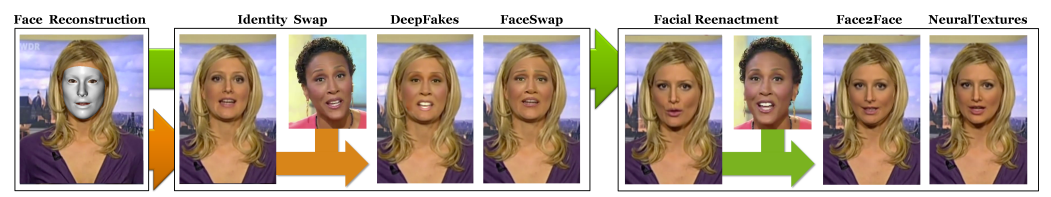
\includegraphics[width=\linewidth]{images/faceforensics.png}
     \captionsetup{font=footnotesize}
     \caption{Procesul de creare a unui DeepFake \cite{rössler2019faceforensics}}
\end{figure}

Setul de date este împărțit în trei subseturi pe baza nivelului de compresie: fără compresie (raw), compresie ușoară (c23) și compresie severă (c40). Acest lucru permite cercetătorilor să testeze robustețea algoritmilor de detecție la diferite niveluri de calitate video.

În lucrarea „Video Face Manipulation Detection Through Ensemble of CNNs”(2020) \cite{bonettini2020video}, autorii abordeaza problema detectării fețelor manipulate în secvențele video, folosind setul FaceForensics++.  Metoda propusă utilizează modelul EfficientNetB4\cite{tan2019efficientnet}, îmbunătățit prin mecanisme de atenție \cite{vaswani2017attention}. Antrenarea modelelor a fost făcută pe seturile de date FaceForensics++ și DeepFake Detection Challenge(o bază de date ce conține peste 119.000 de secvențe din video-uri create pentru o competiție organizată de \href{https://www.kaggle.com/}{Kaggle}. 

\begin{figure}[h]
     \centering 
     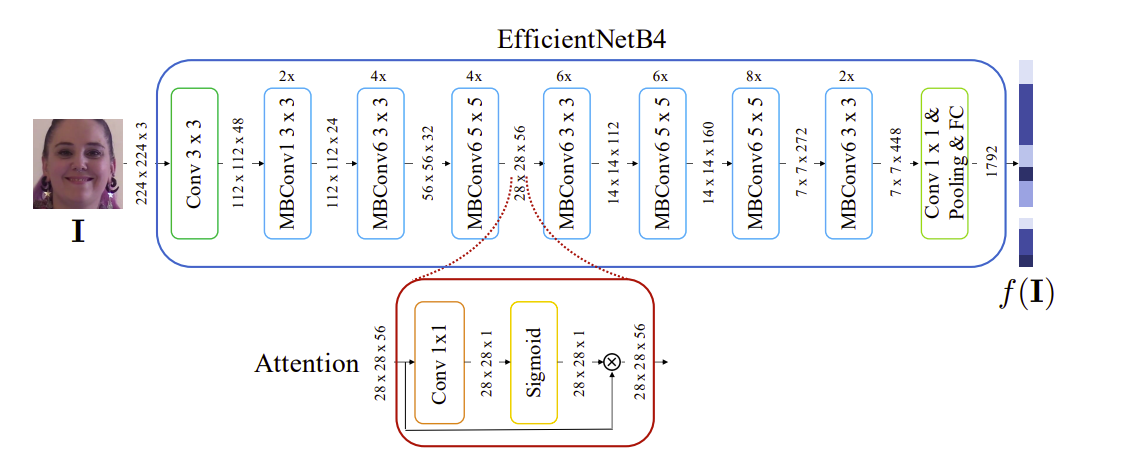
\includegraphics[width=\linewidth]{images/efficientnetb4.png}
     \captionsetup{font=footnotesize}
     \caption{EfficientNetB4 cu atenție \cite{bonettini2020video}}
\end{figure}

Acuratețea modelului a fost evaluată folosind metrica AUC(Area Under Curve), care indică ce capacitate are modelul în a distinge între clasele pozitive și negative.

Autorii au antrenat diverse versiuni ale arhitecturii EfficientNet-B4, pe care în final le-au unit într-un ansamblu de rețele, care a obținut scorul AUC de 0.9444. 

